\chapter{Background}
\label{background}
Explain relevant concepts needed to understand the experiments and findings:\\

Binary Reverse Engineering:
\begin{itemize}
    \item Compilers and compiler levels
    \item Stripping
    \item Ghidra
\end{itemize}

NLP for code:
\begin{itemize}
\item Code Summarization
\item Transformers and CodeT5
\item Scoring methods
\end{itemize}

\newpage
\section{Binary Reverse Engineering}

\subsection{Compilers and Optimization Levels}
Compilers are programs that translate code from one language to another, but generally and in the context of this thesis, the term is used to refer to programs that translate high level code like C to a lower level language such as machine code. For our work we focus on the GNU Compiler Collection (gcc)\footnote{gcc: \url{https://gcc.gnu.org/}} and Clang/LLVM (Clang)\footnote{Clang: \url{https://clang.llvm.org/}}.

Compilers frequently feature optimization levels. Generally the goal of optimizations is the improvement of runtime performance or program size at the expense of compilation time and ability to debug \cite{ColeOptimizationLevel}. Compilers generally use optimizations, grouped into optimization levels, where each level uses a different set of optimizations.

For example, the gcc features 60 optimizations across 8 different optimization levels, which are denoted by a -O option \cite{ColeOptimizationLevel, gccOptimization}. By default, if gcc is invoked without any optimization options, the program will be compiled with O0. O1, 02 and O3 incrementally apply more optimization to the binary at the expense of a higher compilation time \cite{gccOptimization}. These optimization levels are also found in other compilers such as Clang-LLVM. Other optimization levels, such as Os, which optimizes for binary size, are also included in gcc \cite{gccOptimization}.

Optimizations can restructure and transform the program in relation to the source code, by changing the control flow or the data of the program \cite{optimizationObfuscation}. This obfuscation can complicate the reverse engineering process by reducing the accuracy of Ghidra \cite{optimizationObfuscation}.  

\subsection{Ghidra}
Ghidra is a free and open source reverse engineering toolkit developed by the US National Security Agency. Ghidra has been in development since the turn of the century and had been in use internally. Its existence was leaked by Wikileaks in March of 2017 and the tool was released to the public in March of 2019, before being open sourced in April of the same year.

Ghidra contains many separate analysis modules that allow a reverse engineer to analyse compiled code. The modularity of Ghidra and the inclusion of a scripting engine allow users to add custom modules and scripts. We will specifically focus on the tools used in the process that was used to transform binaries into readable code (see \ref{fig:ghidra}).

\label{fig:ghidra}
\begin{figure}[!h]
  \centering
  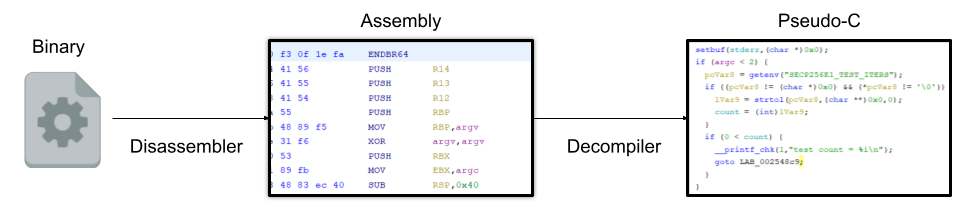
\includegraphics[width=\linewidth]{img/ghidra.png}
  \caption{Transformation of binary to readable code.}
\end{figure}

Ghidra features a disassembler \ref{fig:disassembler}, which will take the binaries and assemble them back into an intermediate representation. In the case of x86-x64 binaries like the binaries this project will focus on, this intermediate representation will be assembly. Processors have an associated language that defines the mapping
between user readable assembly language instructions (e.g. MOV, ADD, etc.) and their corresponding byte values. In order to properly disassemble a binary image for a specific architecture, Ghidra requires a language module for that specific processor. A language module is the software that implements the language translation. Ghidra has a set of language modules for the most popular processor languages(such as x86-64, ARM. MIPS ..). Besides these out-of-the-box supported architectures, developers have also been extending Ghidra's support with custom processor architectures. 
\label{fig:disassembler}
\begin{figure}[!h]
  \centering
  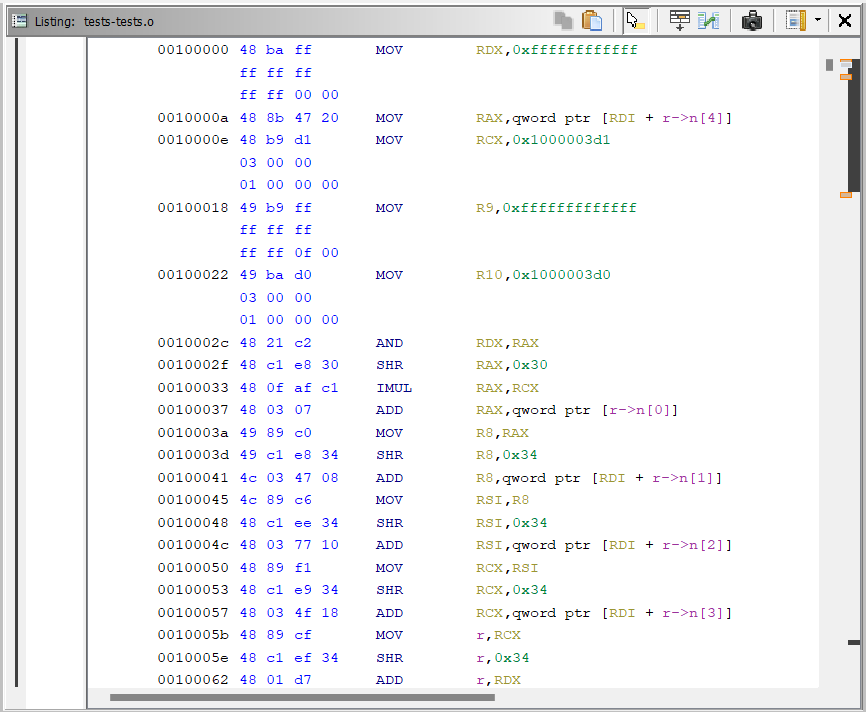
\includegraphics[width=\linewidth]{img/disassembler.png}
  \caption{Ghidra's disassembly window.}
\end{figure}

The decompiler, also featured in Ghidra \ref{fig:decompiler}, is a processor language-agnostic transformation engine that takes the disassembled code and creates a source code representation. The representation is in pseudo-C, a C-like representation that generally follows the general language conventions of C. The interactive decompiler window allows the user to directly see the correspondence between the pseudo-C and assembly representation. The user can also make changes to the decompiled code, such as changing automatically generated variable names and types and adding comments. 

\label{fig:decompiler}
\begin{figure}[!h]
  \centering
  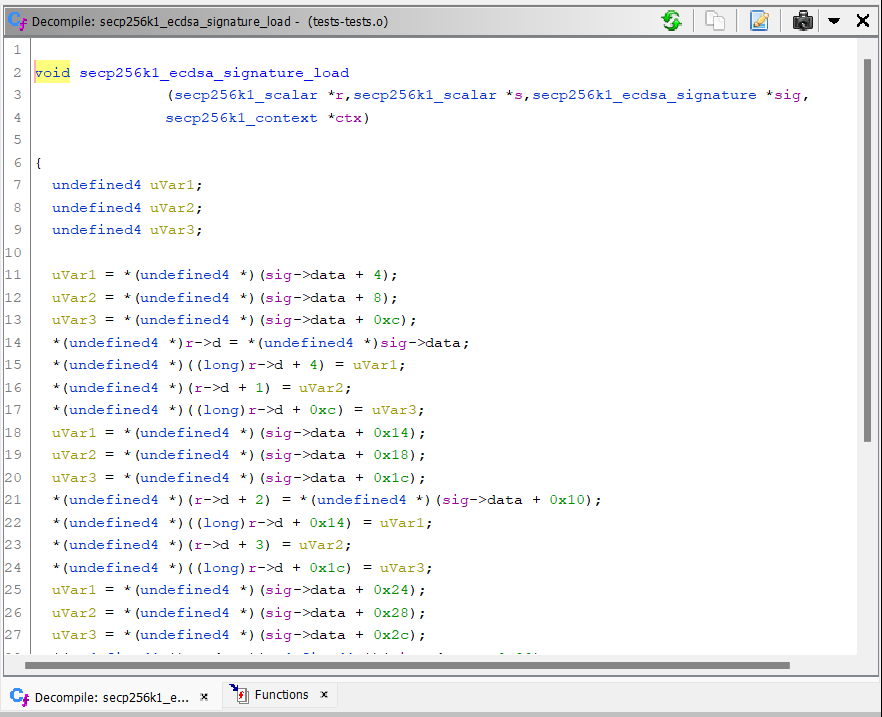
\includegraphics[width=\linewidth]{img/decompiler.png}
  \caption{Ghidra's decompiler window showing a snippet of decompiled function from the secp256k1 ECDSA library}
\end{figure}
\newpage
\subsection{Stripping}
Aside from compiling with higher optimization levels, binaries can also be stripped to obfuscate the underlying code and to resist analysis\cite{StochFuzz}. Binaries which have not been stripped still contain a lot of debug information, which can be used during development. This debug information, like function names, self defined types etc., can be used to analyse and reverse engineer the binary. Commercial Off-the-Shelf (COTS) software is often stripped to reduce the memory and storage footprint of binary, and to resist analysis to protect the intellectual property of the creator. Many vulnerable and malicious binaries are, unfortunately, also stripped to resist security analysis and hide their faults\cite{Debin}.

Unix and Unix-like operating systems include a strip utility. The strip utility removes any operands that are not necessary for the execution for the binary, while ensuring that the execution of the binary remains unchanged, the exact implementation and scope of the utility is left to the implementation\footnote{strip: \url{https://pubs.opengroup.org/onlinepubs/007908799/xcu/strip.html}}. 

The strip utility as implemented in GNU/Linux, removes the symbol table from the binary. The symbol table contains the symbol location, type and name. The symbol table can be dumped for a given binary by using the nm command \ref{fig:nm}, which is included in Unix and Unix-like operating systems \footnote{nm: \url{https://pubs.opengroup.org/onlinepubs/9699919799/utilities/nm.html}}. 

\label{fig:nm}
\begin{figure}[!h]
  \centering
\begin{lstlisting}
                 U malloc
                 U memcpy
                 U memset
0000000000000060 r minus_b1.3052
0000000000000040 r minus_b2.3053
0000000000005680 t nonce_function_rfc6979
00000000000000c1 r one.4283
0000000000000120 r output32.4535
00000000000000e0 r pad.4239
00000000001101e0 r secp256k1_const_lambda
0000000000110240 r secp256k1_const_modinfo_fe
0000000000110200 r secp256k1_const_modinfo_scalar
000000000000c7d0 T secp256k1_context_clone
000000000000c690 T secp256k1_context_create
000000000000c920 T secp256k1_context_destroy
0000000000000000 D secp256k1_context_no_precomp
...
\end{lstlisting}
  \caption{Sample output of nm command from secp256k1 \protect\footnote{Bitcoin secp256k1: \protect\url{https://github.com/bitcoin-core/secp256k1}} ECDSA library}
\end{figure}
% FIX THIS, footnote doesnt work

Like higher optimization levels, the use of stripping can greatly complicate the efforts to reverse engineer a binary, as well as reduce the accuracy and effectiveness of reverse engineering tools. 
\section{NLP for Code}

\subsection{Code Summarization}

\subsection{Transformer and CodeT5}
The current state-of-the-art natural language programming language processing models such as CodeT5 \cite{CodeT5}, CodeBERT \cite{CodeBERT} and CodeX \cite{CodeX} are all based on the Transformer architecture \cite{Transformers}.

Pre-trained language models, such as RoBERTa, CodeBERT \cite{CodeBERT} and CodeT5 \cite{CodeT5} utilize a pre-train and fine-tune paradigm. In this paradigm the models are first trained in an unsupervised manner on a large unlabeled dataset. In the case of RoBERTa, a Masked Language Modeling (MLM) objective was used, where random tokens are masked out from a swath of text (or CodeBERTs case code) and the model is tasked to predict said tokens.

\subsection{Scoring Methods}